\lab{Mayavi}{Mayavi}

\section*{3-D Plotting with Mayavi} % =========================================

Although Matplotlib is capable of creating 3-D plots, Mayavi\footnote{If Mayavi is not installed on your machine, run \li{conda install mayavi} from the command line. See Appendix \ref{updateinstall} for more info.} does it much faster and with better visuals.
Here we introduce methods for plotting space curves, scatter plots, and surfaces in 3-D.
The \li{mlab} submodule within the \li{mayavi} package contains the functions for creating these plots.
% We will use Mayavi for all 3-D plots in these labs. % O RLY?

\begin{warn}
Mayavi must be imported before Matplotlib.
\begin{lstlisting}
from mayavi import mlab
from matplotlib import pyplot as plt
\end{lstlisting}
\end{warn}

\begin{comment}
\begin{info} % Installation note. Make into a footnote?
If you do not have the \li{Mayavi} package installed on your system, you may download it by running the following commands from the command line:
\begin{lstlisting}
$ conda install conda               # Download the most recent installer.
$ conda install anaconda            # Update all packages.
$ conda install mayavi              # Installs mayavi.
\end{lstlisting}

% For more information regarding installing Python packages, see Appendix \ref{updateinstall}.
\end{info}

\begin{table} % Mayavi plotting functions. Probably should put this back in.
\begin{center}
\begin{tabular}
{|c|l|}
\hline
Function & Description \\
\hline
\li{barchart} & Produces 3D histogram-like plots\\
\li{contour3d} & Plots level surfaces of functions of three variables\\
\li{flow} & Creates a trajectory of particles following the flow of a vector field\\
\li{imshow} & Use a colormap to view a 2D array as an image\\
\li{mesh} & Plot a surface using \li{(x,y,z)} coordinates supplied as three 2D arrays\\
\li{plot3d} & Draws lines between points\\
\li{points3d} & Plots glyphs (like points) at the coordinates supplied\\
\li{quiver3d} & Generate 3D vector fields\\
\li{surf} & Plot a surface with a 2D array as elevation data\\
\hline
\end{tabular}
\end{center}
\caption{Some plotting functions in \li{mlab}.}
\label{table:mlab_functions}
\end{table}
\end{comment}

\subsection*{Lines} % ---------------------------------------------------------

The function \li{mlab.plot3d()} is the 3-D Mayavi equivalent for Matplotlib's \li{plt.plot()}.
Because the plot is 3-D, we must provide $x$, $y$, and $z$ coordinates, each contained in 1-D arrays of the same length.
The points \li{(x[i], y[i], z[i])} are graphed in $\mathbb{R}^3$ and connected with straight lines.

Consider the following curve, parametrized by time:
\begin{align*}
x(t) &= \cos(t)(1+\cos(6t))\\
y(t) &= \sin(t)(1+\sin(6t)\\
z(t) &= \sin\left(\frac{6}{11}t\right)
\end{align*}
The following code plots the curve over the time domain $t \in [0,2\pi]$.
The resulting plot is shown in Figure \ref{fig:plot3d}.

\begin{lstlisting}
>>> from mayavi import mlab

# Calculate the coordinates of a curve parametrized by time.
>>> t = np.linspace(0, 2*np.pi, 100)
>>> x = np.cos(t) * (1 + np.cos(t*6))
>>> y = np.sin(t) * (1 + np.cos(t*6))
>>> z = np.sin(t*6/11.)

# Plot and show the figure.
>>> mlab.plot3d(x, y, z)
>>> mlab.show()
\end{lstlisting}

\begin{figure} % Mayavi line and point plots.
\captionsetup[subfigure]{justification=centering}
\centering
\begin{subfigure}{.5\textwidth}
    \centering
    
\includegraphics[width=\linewidth]{plot3d.png}
    \caption{A 3-D curve generated by \li{mlab.plot3d()}.}
    \label{fig:plot3d}
\end{subfigure}%
\begin{subfigure}{.5\textwidth}
    \centering
    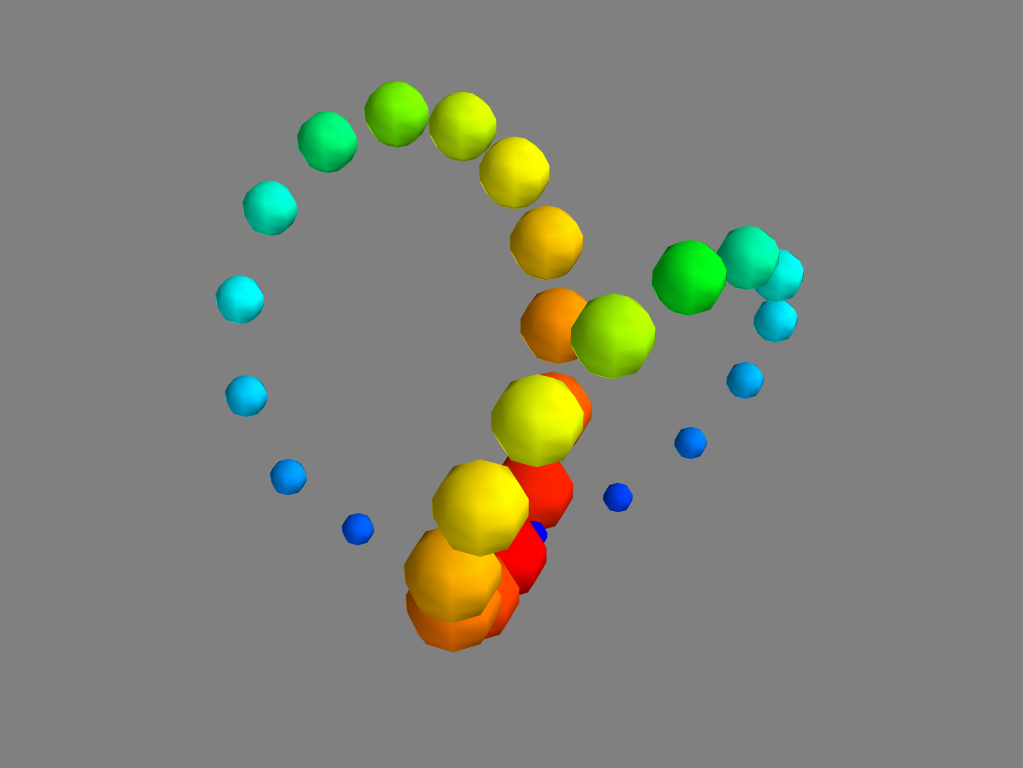
\includegraphics[width=\linewidth]{points3d.png}
    \caption{A 3-D scatter plot generated by \li{mlab.points3d()}.}
    \label{fig:points3d}
\end{subfigure}
\end{figure}

\subsection*{Points} % --------------------------------------------------------

The function \li{mlab.points3d()} is the 3-D Mayavi equivalent for Matplotlib's \li{plt.scatter()}.
Each point is plotted, but not connected with lines.
In the code below, the optional input array \li{s} defines a scalar for each point that modifies the color and size of the point.
The output is in Figure \ref{fig:points3d}.

\begin{lstlisting}
>>> t = np.linspace(0, 4*np.pi, 30)
>>> x = np.sin(2*t)
>>> y = np.cos(t)
>>> z = np.cos(2*t)
>>> s = 2 + np.sin(t)

# Adjust the keyword argument 'scale_factor' so all points are visible.
>>> mlab.points3d(x, y, z, s, scale_factor=.15)
>>> mlab.show()
\end{lstlisting}

\subsection*{Surfaces} % ------------------------------------------------------

The function \li{mlab.surf()} renders a 3-D surface.
Because the surface is over a 2-D domain, we create a coordinate grid with \li{np.mgrid()} (similar to \li{np.meshgrid()}).
This function uses the slicing syntax \li{[start:stop:step]}, similar to \li{range()} and \li{np.arange()}, but is accessed with brackets instead of parentheses.

The following code produces the hyperbolic paraboloid $f(x,y) = \frac{x^2}{4} - \frac{y^2}{4}$ over the domain $[-4,4]\times[-4,4]$.
The result is displayed in Figure \ref{fig:surf_example}.

\begin{lstlisting}
>>> X, Y = np.mgrid[-4:4:.025, -4:4:.025]
>>> Z = (X**2)/4. - (Y**2)/4.
>>> mlab.surf(X, Y, Z, colormap='RdYlGn')
>>> mlab.show()
\end{lstlisting}

\begin{figure}
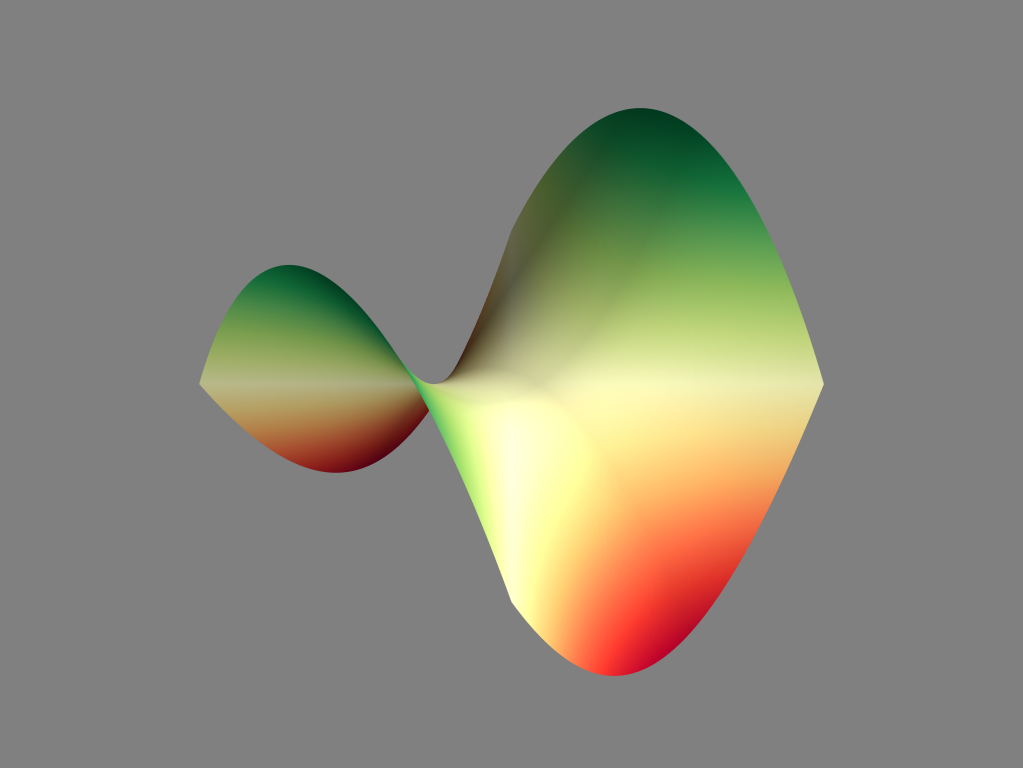
\includegraphics[width=.7\textwidth]{mesh_example.png}
\caption{Sample output of \li{mlab.surf()}.}
\label{fig:surf_example}
\end{figure}

Like Matplotlib, Mayavi supports various color schemes, either as a solid color or with a varying colormap.
For example, the plot in Figure \ref{fig:surf_example} uses the colormap \li{'RdYlGn'}.
For a list of all colormaps in Mayavi, see \url{http://docs.enthought.com/mayavi/mayavi/mlab_changing_object_looks.html}.

% TODO: More exercises with Mayavi!!! Don't have to be too hard either...
\begin{problem}
Plot the function $z = \frac{1}{10}\sin(10(x^2+y^2))$ on $[-1,1] \times [-1,1]$ using Mayavi.
\end{problem}
